
\section{Jesron Marudut Hatuan/1164077}
\subsection{Teori}
\begin{enumerate}
\item Mengapa file suara harus di lakukan MFCC.
\subitem Alasan mengapa File suara atau audio harus dilakukan MFCC  karena MFCC dapat mengubah file suara/frekuensi suara ke dalam sebuah bentuk data, yaitu menjadi data vektor yang nantinya dapat diolah menjadi sebuah output dimana telah dilakukan ekstraksi oleh MFCC selanjutnya direalisasikan sebagai data matrix. Contoh ilustrasi dapat dilihat pada gambar \ref{c6t_1}.
\begin{figure}[!htbp]
\centerline{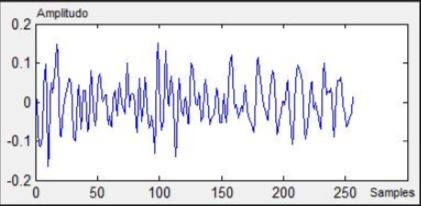
\includegraphics[width=1\textwidth]{figures/c6t/1.JPG}}
\caption{Suara ke MFCC}
\label{c6t_1}
\end{figure} 
\item Penjelasan tentang konsep dasar neural network.
\subitem Neural Network merupakan cara untuk menkomputasi yang efisien dimana tema utamanya dipinjam dari analogi jaringan saraf biologis. Neural Network juga biasa disebut dengan jaringan saraf tiruan dimana Neural Network sebenarnya dapat mengadopsi dari kemampuan otak manusia yang dapat memberikan rangsangan, melakukan proses, dan memberikan output. Contoh ilustrasi dapat dilihat pada gambar \ref{c6t_2}.
\begin{figure}[!htbp]
\centerline{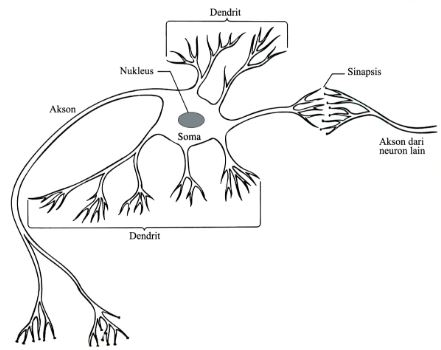
\includegraphics[width=1\textwidth]{figures/c6t/2.JPG}}
\caption{Neural Network}
\label{c6t_2}
\end{figure} 
\item Penjelasan tentang konsep dari pembobotan dalam neural network.
\subitem Neural Network dapat dikonfigurasi untuk aplikasi tertentu, seperti pengenalan pola atau klasifikasi data, contohnya saat Neural Network melakukan penyesuaian koneksi sinaptik antara Neuron, maka dilakukan dengan menyesuaikan nilai bobot yang ada pada setiap konektivitas baik dari input, Neuron maupun output disinkronkan dengan penyesuaian koneksi sinaptik antar neuron itu sendiri. Contoh ilustrasi dapat dilihat pada gambar \ref{c6t_3}.
\begin{figure}[!htbp]
\centerline{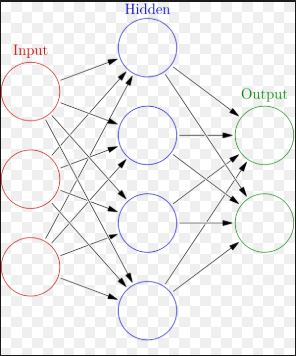
\includegraphics[width=1\textwidth]{figures/c6t/3.JPG}}
\caption{Konsep Pembobotan pada Neural Network}
\label{c6t_3}
\end{figure} 
\item Penjelasan tentang konsep fungsi aktifasi dalam Neural Network.
\subitem Dalam Neural Network, fungsi aktivas adalah setiap Neuron dapat mempunyai tingkat aktivasi yang merupakan fungsi dari input yang masuk padanya. Aktivasi yang dikirim suatu Neuron ke Neuron lain berupa sinyal dan hanya dapat mengirim sekali dalam satu waktu, meskipun sinyal tersebut disebarkan pada beberapa neuron yang lain. Contoh ilustrasi dapat dilihat pada gambar \ref{c6t_4}.
\begin{figure}[!htbp]
\centerline{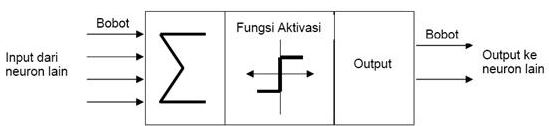
\includegraphics[width=1\textwidth]{figures/c6t/4.JPG}}
\caption{Fungsi Aktivasi pada Neural Network}
\label{c6t_4}
\end{figure} 
\item Penjelasan cara membaca hasil plot dari MFCC.
\subitem Cara membaca dari MFCC yaitu nanti akan ada outputan berbentuk grafik setelah melakukan plot dari MFCC. Kemudian terdapat frekuensi/Hz pada suara frekuensi biasanya vertikal atau biasa disimbolkan dengan sumbu y, Lalu terdapat waktu yang mana waktu diartikan dalam simbol sumbu x. Sedangkan pada bagian dalam dapat disimbolkan dengan sumbu z yang merupakan power atau kekuatan dari lagu atau suara atau audio yang dihasilkan. Untuk warna biru itu merupakan suara rendah, yang merah merupakan tinggi apabila daya frekuensi nya misalkan suara siul berarti dominan warna merah karena siul biasanya pada nada yang tinggi sedangkan jika bass dominan biru karena bass merupakan nada rendah. Contoh ilustrasi dapat dilihat pada gambar \ref{c6t_5}.
\begin{figure}[!htbp]
\centerline{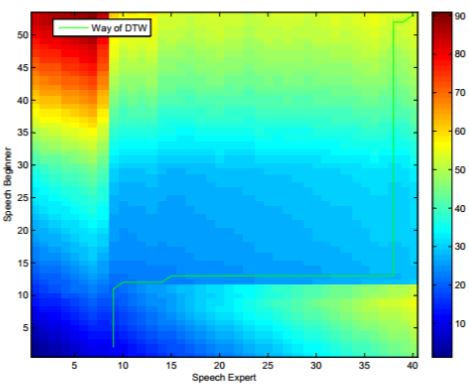
\includegraphics[width=1\textwidth]{figures/c6t/5.JPG}}
\caption{Membaca Hasil Plot dari MFCC}
\label{c6t_5}
\end{figure} 
\item Penjelasan tentang apa itu one-hot encoding.
\par One-hot encoding yaitu sebuah caraa untuk representasi data dari variabel kategori sebagai vektor biner. Yaitu nilai kategorika harus dipetakan ke nilai integer. Selanjutnya, setiap nilai integer direpresentasikan sebagai vektor biner yang semuanya bernilai nol kecuali indeks integer, yang dapat ditandai dengan 1. Contoh ilustrasi dapat dilihat pada gambar \ref{c6t_6}.
\begin{figure}[!htbp]
\centerline{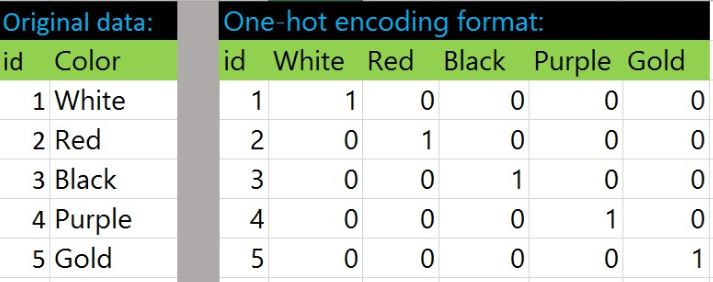
\includegraphics[width=1\textwidth]{figures/c6t/6.JPG}}
\caption{One-Hot Encoding}
\label{c6t_6}
\end{figure} 
\item Penjelasan fungsi dari np.unique dan to\_categorical dalam kode program.
\begin{itemize}
\item np.unique adalah cara untuk mengekstaksi elemen-elemen unik tertentu yang terdapat dalam array.
\item sedangkan to\_categorical adalah cara untuk mengubah vektor kelas yang berupa integer menjadi matriks kelas biner.
\end{itemize}
\begin{figure}[!htbp]
\centerline{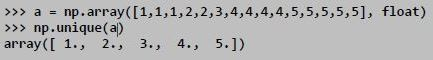
\includegraphics[width=1\textwidth]{figures/c6t/7.JPG}}
\caption{np.unique}
\end{figure} 
\begin{figure}[!htbp]
\centerline{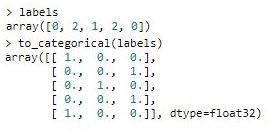
\includegraphics[width=1\textwidth]{figures/c6t/7_1.JPG}}
\caption{to\_categorical}
\end{figure} 
\item Penjelasan fungsi dari Sequential dalam kode program.
\subitem Fungsi dari Sequential dalam kode program yaitu sebuah jenis model yang dapat digunakan dalam perhitungan ataupun code program yang dapat direalisasikan. Neural Networks Sequential dapat membangun fitur tingkat tinggi melalui lapisan yang berurutan. Sequential juga merupakan proses dimana membandingkan setiap elemen larik satu per satu secara beruntun, mulai dari elemen pertama, sampai dengan elemen terakhir atau elemen yang dicari sudah ditemukan.  Contoh ilustrasi dapat dilihat pada gambar \ref{c6t_8}.
\begin{figure}[!htbp]
\centerline{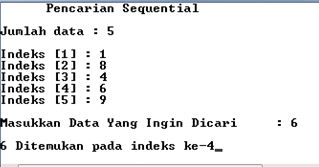
\includegraphics[width=1\textwidth]{figures/c6t/8.JPG}}
\caption{One-Hot Encoding}
\label{c6t_8}
\end{figure} 
\end{enumerate}


\subsection{Praktek Program}
\begin{enumerate}
\item Penjelasan dari data GTZAN Genre Collection dan data dari freesound dan Berupa kode program untuk meload data tersebut untuk digunakan pada MFCC.
\subitem Isi dari data GTZAN Genre Collection itu isinya berupa data musik yang sudah di folderkan berdasarkan genre lagunya (dikelompokkan) dengan ekstensi .au yang akan kita lakukan proses MFCC. Sedangakan freesound hanya untuk 1 lagu saja dengan ekstensi .wav.
\lstinputlisting[firstline=1, lastline=2]{src/Jazz.py}
\begin{itemize}
\item Code pada baris pertama yaitu Filename jazz merupakan sebuah variabel yang nantinya berisikan direktori dari file yang dituju, pada code ini digunakan file audio dari genre jazz.
\item Code pada baris kedua yaitu membuat variabel X jazz dan sr jazz yang digunakan untuk meload file dari variabel filename jazz menggunakan librari Librosa dengan durasi 10, yang nantinya akan digunakan pada Mfcc.
\end{itemize}
\subitem Hasilnya dapat dilihat pada gambar \ref{c6t_9}.
\begin{figure}[!htbp]
\centerline{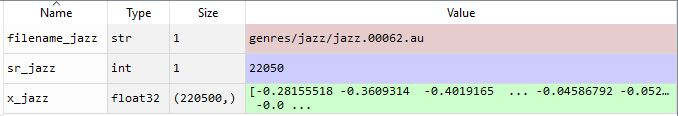
\includegraphics[width=1\textwidth]{figures/c6t/9.JPG}}
\caption{GTZAN}
\label{c6t_9}
\end{figure} 
\item Penjelasan perbaris kode program dengan kata-kata dan dilengkapi ilustrasi gambar fungsi dari display mfcc() .
\lstinputlisting[firstline=42, lastline=42]{src/Genreidentifier.py}
\subitem Pada kode tersebut menjelaskan display\_mfcc untuk menampilkan vektorisasi dari sebuah suara yang akan menampilkan Plot dan Bar dari inputan code dan file suara hiphop.00028.au. Hasilnya dapat dilihat pada gambar \ref{c6t_10}.
\begin{figure}[!htbp]
\centerline{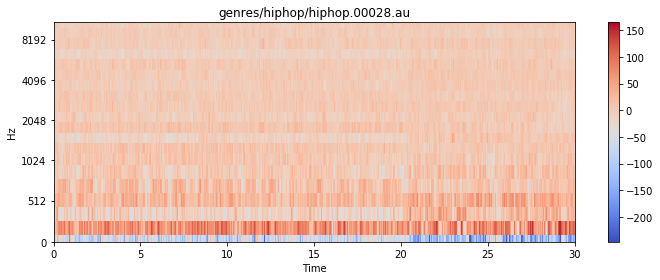
\includegraphics[width=1\textwidth]{figures/c6t/10.png}}
\caption{Display MFCC}
\label{c6t_10}
\end{figure} 
\item Penjelasan perbaris kode program dengan kata-kata dan dilengkapi ilustrasi gambar fungsi dari extract features song(). Jelaskan juga mengapa yang diambil 25.000 baris pertama?
\lstinputlisting[firstline=42, lastline=42]{src/Genreidentifier.py}
\begin{itemize}
\item Pada kode baris pertama berfungsi untuk memuat inputan. 
\item Pada kode baris kedua itu akan memuat data inputan dengan menggunakan librosa.
\item Kemudian pada parameter inputan yaitu y untuk membuat sebuah fitur pada mfcc.
\item Selanjutnya me-return menjadi array dan akan mengambil 25000 data saja dari hasil vektorisasi dalam 1 lagu yang sudah di display\_mfcc.  
\item Mengapa yang dimabil 25.000 baris pertama karena nemuat nilai-nilai MFCC untuk lagu, tetapi karena nilai-nilai ini mungkin antara negatif 250 hingga positif 150, mereka tidak baik untuk jaringan saraf.
\end{itemize}
\item Penjelasan perbaris kode program dengan kata-kata dan dilengkapi ilustrasi gambar fungsi dari generate features and labels().
\lstinputlisting[firstline=58, lastline=75]{src/Genreidentifier.py}
\subitem Pada kode diatas berfungsi melakukan fungsi yang sebelumnya kita telah jalankan. Lalu pada bagian genres itu disesuaikan dengan nama folder dataset. Untuk baris selanjutnya itu akan melakukan looping dari folder genres dengan ektensi .au. Lalu akan memanggil fungsi ekstrak lagu. Pada setiap file yang terdapat pada folder itu akan di ekstrak menjadi vektor dan akan dimasukan kedalam fitur. Dan fungsi append itu menumpuk file-file yang telah di vektorisasi.
\item Penjelasan dengan kata dan praktek kenapa penggunaan fungsi generate features and labels() sangat lama ketika meload dataset genre.
\lstinputlisting[firstline=79, lastline=79]{src/Genreidentifier.py}
\subitem Pada kode diatas menjelaskan dikarenakan terdapat 10 folder dengan genre berbeda, dan didalamnya terdapat 100 audio maka itu akan lama untuk meload dataset genre. Dari setiap folder itu akan dilakukan features dan perubahan label dengan ekstrasi data mengunakan mfcc. Karena banyaknya jumlah file maka proses loadnya pun lama. Hasil dapat dilihat pada gambar \ref{c6t_11}.
\begin{figure}[!htbp]
\centerline{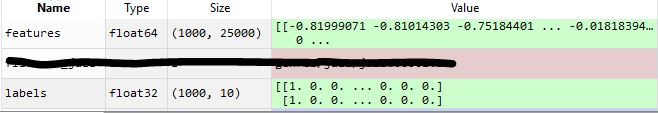
\includegraphics[width=1\textwidth]{figures/c6t/11.JPG}}
\caption{Generate Features and Labels}
\label{c6t_11}
\end{figure}
\item Penjelasan kenapa harus dilakukan pemisahan data training dan data set sebesar 80 persen?
\lstinputlisting[firstline=84, lastline=84]{src/Genreidentifier.py}
\subitem Pada kode diatas berfungsi untuk memisahkan data training dan dataset sebesar 80\% digunakan untuk memudahkan dalam melakukan pengacakan atau pengocokan nantinya. Dimana 80\% merupakan data training dan sisanya 20\% merupakan datatestnya. data training perlu lebih banyak agar saat dilakukan pengocokan tidak teracak dalam urutan yang berbeda. Hasilnya dapat dilihat pada gambar \ref{c6t_12}.
\begin{figure}[!htbp]
\centerline{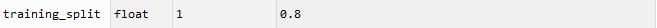
\includegraphics[width=1\textwidth]{figures/c6t/12.JPG}}
\caption{Training Data Sebesar 80\%}
\label{c6t_12}
\end{figure}
\item Mempraktekkan dan jelaskan masing-masing parameter dari fungsi Sequential().
\lstinputlisting[firstline=106, lastline=111]{src/Genreidentifier.py}
\subitem Pada kode diatas dijelaskan bahwa:
\begin{itemize}
\item Layer pertama dense dari 100 neuron untuk inputan
\item Activationnya menggunakan fungsi relu yaitu jika ada inputan dengan nilai maksimum maka inputan itu yang akan terpilih.
\item Dense 10 mengkategorikan 10 neuron untuk jenis genrenya untuk output nya.
\item Untuk dense diatas aktivasinya menggunakan fungsi Softmax
\end{itemize}
\item Praktekkan dan jelaskan masing-masing parameter dari fungsi compile() dan tunjukkan keluarannya dengan fungsi summary.
\lstinputlisting[firstline=113, lastline=116]{src/Genreidentifier.py}
\subitem Pada kode diatas dijelaskan bahwa:
\begin{itemize}
\item Menggunakan algortima adam sebagai optimizer. Adam yaitu algoritme pengoptimalan yang dapat digunakan sebagai ganti dari prosedur penurunan gradien stokastik klasik untuk memperbarui bobot jaringan yang berulang berdasarkan data training.
\item Loss nya menggunakan categorical\_crossentropy untuk fungsi optimasi skor
\end{itemize}
\subitem Hasilnya dapat dilihat pada gambar \ref{c6t_13}.
\begin{figure}[!htbp]
\centerline{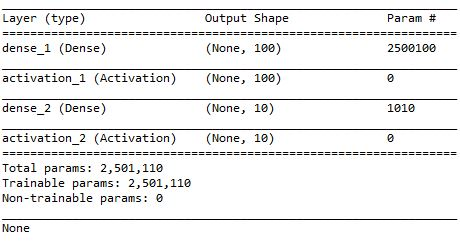
\includegraphics[width=1\textwidth]{figures/c6t/13.JPG}}
\caption{Fungsi Compile}
\label{c6t_13}
\end{figure}
\item Penjelasan dan jelaskan masing-masing parameter dari fungsi fit().
\lstinputlisting[firstline=118, lastline=119]{src/Genreidentifier.py}
\subitem Pada kode tersebut dapat dilihat bahwa pada model fit digunakan untuk melatih mesin dengan data training input dan training label. Epochs ini merupakan iterasi atau pengulangan berapa kali data tersebut akan dilakukan. Batch\_size ini adalah jumlah file yang akan dilakukan pelatihan pada setiap 1 kali pengulangan. Sedangkan validation\_split itu untuk menentukan presentase dari cross validation atau k-fold sebanyak 20\% dari masing-masing data pengulangan. Hasilnya dapat dilihat pada gambar \ref{c6t_14}.
\begin{figure}[!htbp]
\centerline{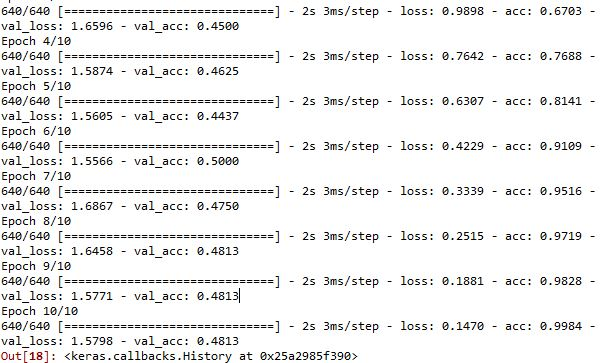
\includegraphics[width=1\textwidth]{figures/c6t/14.JPG}}
\caption{Fungsi Fit}
\label{c6t_14}
\end{figure}
\item Mempraktekkan dan jelaskan masing-masing parameter dari fungsi evaluate().
\lstinputlisting[firstline=121, lastline=121]{src/Genreidentifier.py}
\subitem Pada kode diatas maka dapat dilihat bahwa dengan menggunakan test input dan test label dilakukan evaluasi atau proses menemukan model terbaik yang mewakili data dan seberapa baik model yang dipilih akan dijalankan kedepannya. Hasilnya dapat dilihat pada gambar \ref{c6t_15}.
\begin{figure}[!htbp]
\centerline{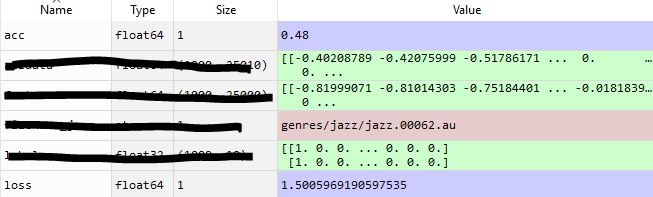
\includegraphics[width=1\textwidth]{figures/c6t/15.JPG}}
\caption{Fungsi Evaluate}
\label{c6t_15}
\end{figure}
\item Praktekkan dan jelaskan masing-masing parameter dari fungsi predict(). 
\lstinputlisting[firstline=127, lastline=127]{src/Genreidentifier.py}
\subitem Pada kode diatas akan melakukan testing satu data lagu. file yang di jalankan tersebut termasuk ke dalam genre apa, hasilnya bisa dilihat pada gambar tersebut presentase yang paling besar yakni genre hiphop. Maka lagu tersebut termasuk ke dalam genre hiphop dengan perbandingan presentase hasil prediksi. Hasilnya dapat dilihat pada gambar \ref{c6t_16}.
\begin{figure}[!htbp]
\centerline{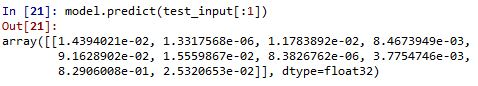
\includegraphics[width=1\textwidth]{figures/c6t/16.JPG}}
\caption{Fungsi Predict}
\label{c6t_16}
\end{figure}
\end{enumerate}

\subsection{Penanganan Eror}
\begin{enumerate}
\item ScreenShoot Error dapat dilihat pada gambar \ref{c6t_17}.
\begin{figure}[!htbp]
\centerline{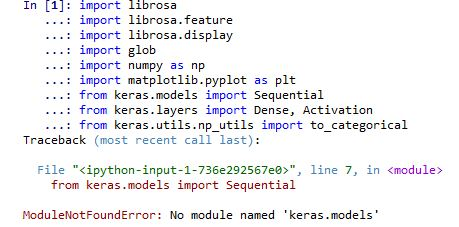
\includegraphics[width=1\textwidth]{figures/c6t/eror.JPG}}
\caption{Eror}
\label{c6t_17}
\end{figure}
\item Tuliskan kode eror dan jenis errornya.
\lstinputlisting[firstline=131, lastline=131]{src/Genreidentifier.py}
\item Solusi pemecahan masalah error tersebut.
\lstinputlisting[firstline=133, lastline=139]{src/Genreidentifier.py}
\end{enumerate}